

\section{Grundlagen}
\begin{itemize}
    \item \textbf{Transkriptom}: %K
    Summe der zu einem bestimmten Zeitpunkt in einer Zelle transkribierten, das heißt von der DNA in RNA umgeschriebenen Gene, also die Gesamtheit aller in einer Zelle hergestellten RNA-Moleküle \index{Transkriptom}
    \item \textbf{Transkriptomik}: %K
    Studie der (m)RNA-Expression einer Zelle \index{Transkriptomik} 
\begin{itemize} 
    \item \textbf{Vorteile}:%K
    Genexpression in Zellen oder Geweben quantifizieren ->detaillierten Überblick darüber, welche Gene unter bestimmten Bedingungen aktiv sind und in welchem Ausmaß
    \item \textbf{Limitierungen}:%K
    erzeugt riesige Mengen an Informationen, können nicht alle Arten von RNA mit gleicher Effizienz erfassen, inhomogene Zellpopulationen können die Ergebnisse verfälschen
\end{itemize}
\end{itemize}
\begin{figure}[H]
\centering
    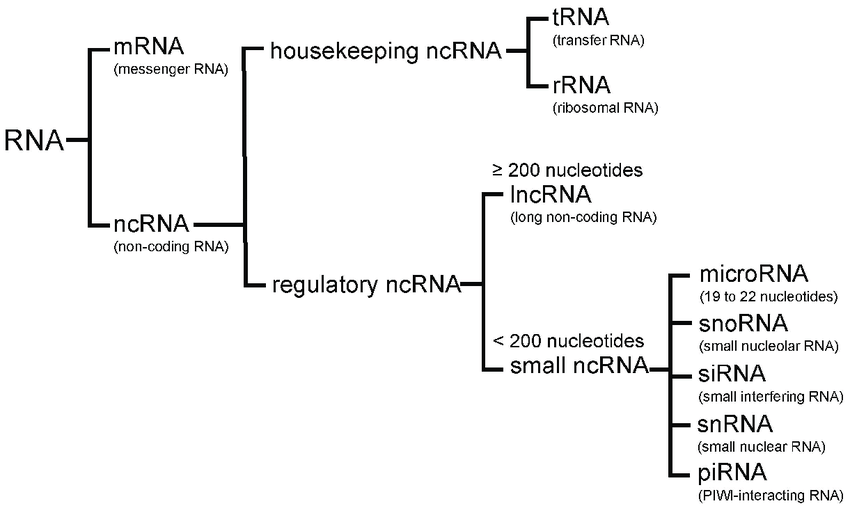
\includegraphics[width=12cm]{images/rnaspecies.png}
    \caption{Zusammenhang der verschiedenen RNA-Typen.}
    \label{fig:rnaspecies}
\end{figure}
\begin{table}[H] %K
    \centering
    \begin{tabular}{|p{2cm}p{2cm}p{3cm}p{1cm}p{6cm}|} \hline
       \textbf{Typ} &  \textbf{Spezies} & \textbf{Zustand} & \textbf{Anteil (\%)}  & \textbf{Aufgabe} \\ \hline \hline 
        coding &  mRNA & nukleare Vorläufer & 6  &  kopiert die in einem Gen auf der DNA liegende Information und trägt sie zum Ribosom, wo mit Hilfe dieser Information die Proteinbiosynthese stattfinden kann \\
        & & Zytoplasmatisch & 3 & \\ \hline
      &   rRNA & nukleare Vorläufer & 4 & trägt keine genetische Information, sondern ist am Aufbau des Ribosoms beteiligt \\
       & & Zytoplasmatisch & 71 & \\  \hline
       &  tRNA & nukleare Vorläufer & 1  & amino acid activation \\
       & & Zytoplasmatisch & 15 & \\ \hline \hline
      non-coding & snRNA & &  & processing of pre-mRNA \\
      & snoRNA & & & processing of pre-mRNA \\
      & miRNA & & & Regulation zellulärer Prozesse, Genregulation,  \gls{Gen-Silencing}  \\
      & siRNA & & & Genregulation, \gls{Gen-Silencing}, \gls{RNA-Interferenz}, Verteidigung gegen fremde RNA   \\
      & lncRNA & & & regulation of gene expression \\
      & circRNA &  & & durch Bindung an miRNA an der Genregulation beteiligt \\ \hline 
    \end{tabular}
    \caption{Vergleich der RNA-Spezies einer Zelle.}
    \label{tab:rnaspezies}
\end{table} \index{RNA!circRNA}\index{RNA!mRNA}  \index{RNA!miRNA} \index{RNA!siRNA}
\index{RNA!lnRNA} \index{RNA!snoRNA} \index{RNA!rRNA} \index{RNA!tRNA}
\begin{mechanism}[title=Unterschied zwischen miRNA und siRNA]
 \textbf{miRNAs} regulieren die Genexpression, indem sie an die \glspl{3utr} von Ziel-mRNAs binden und \textbf{siRNAs} wirken in der Regel durch die \textit{gezielte Zerschneidung} von komplementären mRNAs.  \\
 Daher können siRNAs auch gezielt gegen fremde RNA verteidigen (Infektion durch ein \gls{RNA-Virus}).  \index{RNA-Virus}
\end{mechanism}

\begin{mybox}[title=Unterschied zwischen Genregulation und Regulation der Genexpression] %K
Werden teils synonym verwendet. 
\begin{itemize}
    \item \textbf{Genregulation}: Alle Prozesse, die die Funktion und Aktivität von Genen beeinflussen
    \item \textbf{Regulation der Genexpression}: Die Prozesse, die die Umwandlung von genetischer Information in funktionelle Produkte betreffen (Spezialisierung der Genregulation)
\end{itemize}
\end{mybox}
\begin{mybox}[title=Was macht der Poly-A-Schwanz nochmal?]%K
Gibt Stabilität, ist wichtig für den Export der mRNA aus dem Zellkern, erleichtert die Bindung von Proteinen, die die Initiation der Proteinsynthese unterstützen und fungiert als Signal für die Beendigung der Transkription. 
\end{mybox} \index{Poly-A-Schwanz}
\section{RNA-Verfahren}
\subsection{Isolierung von RNA}
\subsubsection{single step - Methode} \index{RNA-Isolation}
\begin{figure}[H]%K
\centering
    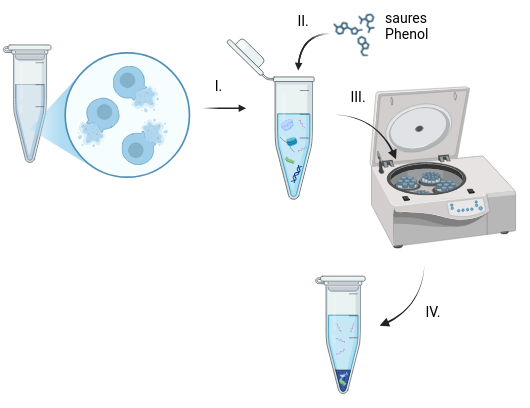
\includegraphics[width=12cm]{images/onestepRNAisolation.png}
    \caption{\textbf{single step RNA-Isolation}: Zellen werden in \gls{gtc} lysiert (I), was die Proteine denaturiert. Durch die Zugabe von saurem \gls{Phenol} (II) und anschließender Zentrifugation (III) werden die DNA und Proteine entfernt. Das geschieht dadurch, dass sie sich sammeln und von der RNA in der wässrigen Phase abtrennen (IV). Man erhält die Gesamt-RNA.}
    \label{fig:onestepRNAisolation}
\end{figure}
\begin{table}[H]%K
    \centering
    \begin{tabular}{p{5cm}p{5cm}}
        \textbf{DNAsen} & \textbf{RNAsen}  \\
        oft nicht temperaturstabil &  temperaturstabil \\
         brauchen oft Cofaktor & benötigen keinen Cofaktor \\
         & „überall vorhanden“ \\
         wenig empfindlich gegenüber DEPC & sensitiv gegen Diethylpyrocarbonat (DEPC) 
    \end{tabular}
    \caption{Vergleich zwischen DNAsen und RNAsen.}
    \label{tab:dnasenrnasen}
\end{table} \index{RNAse} \index{DNAse}
\subsubsection{mRNA isolieren} \index{RNA-Isolation!mRNA-Isolation}
\begin{figure}[H]%K
\centering
    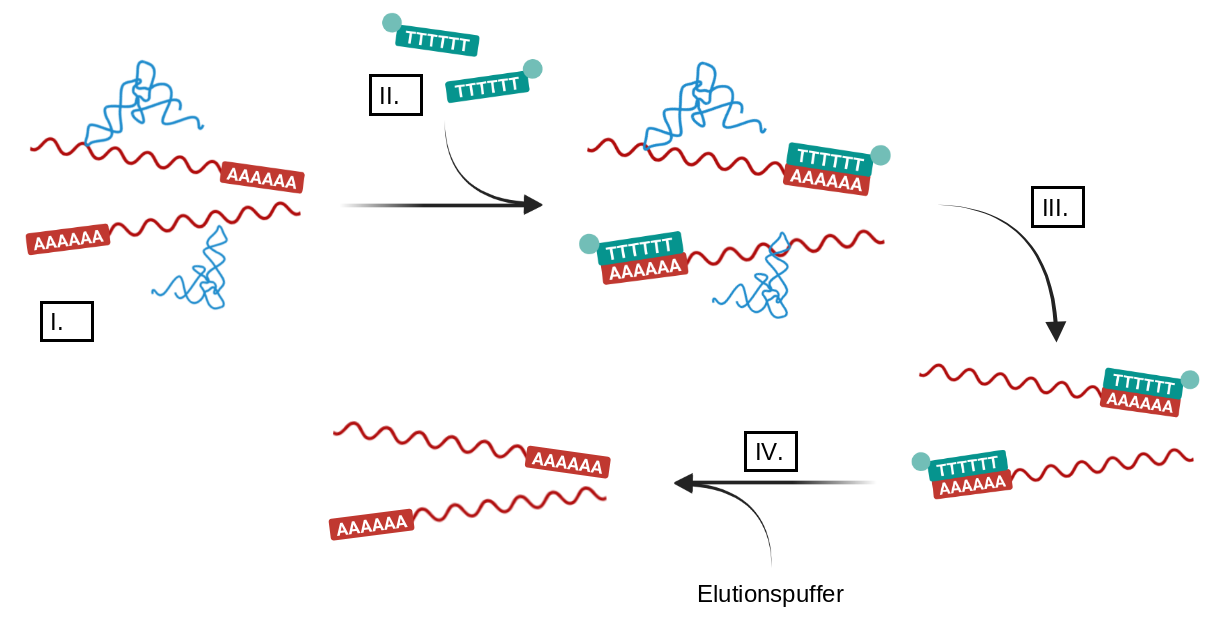
\includegraphics[width=\textwidth]{images/rnaoligoisolation.png}
    \caption{\textbf{mRNA-Isolation}: Der isolierten Gesamt-RNA (I) werden \glspl{Oligo-dT-Sequenz} (grün) hinzugegeben (II). Die Poly-A-Schwänze der mRNA (rot) binden an die Oligo-dT-Sequenzen und können dadurch von dem Rest der RNA getrennt werden (III). Bspw. durch die Verwendung von Mikrokügelchen - es wird sozusagen alles weggewaschen, was nicht an den Oligo-dT-Sequenzen hängt. Anschließend wird die mRNA m.H.v. \gls{Elutionspuffer} von den Oligo-dT-Sequenzen gelöst (IV).} \index{Oligo-dT-Sequenz} \index{Poly-A-Schwanz} \index{Mikrokügelchen}
    \label{fig:rnaoligoisolation}
\end{figure}
\subsubsection{Magnetic Beads} 
\begin{figure}[H]%K
\centering
    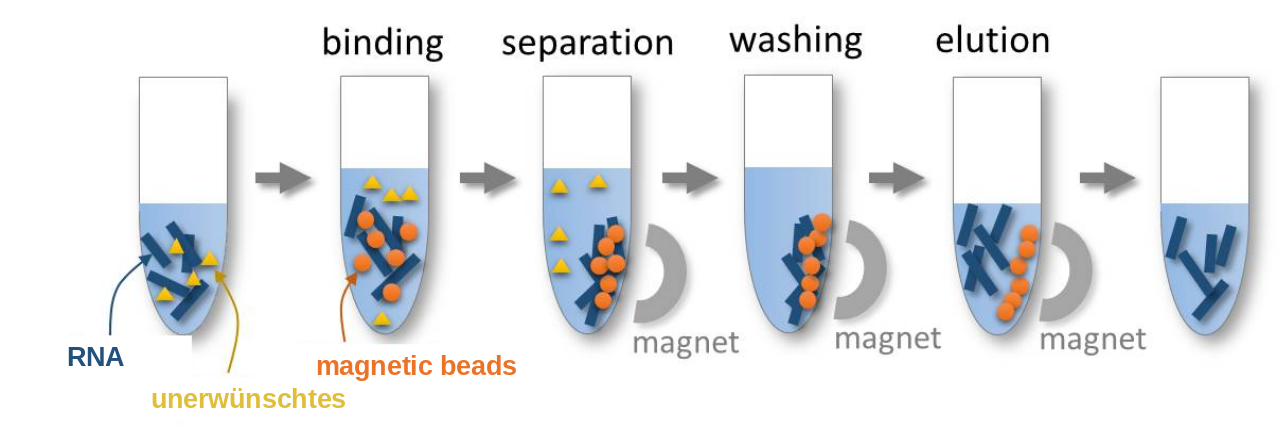
\includegraphics[width=\textwidth]{images/rnabeads.png}
    \caption{\textbf{RNA-Isolation mit magnetischen Mikrokügelchen}: Den lysierten Zellen werden beschichtete magentische Mikrokügelchen hinzugegeben, an die die Ziel-RNA bindet. Es wird ein Magnetfeld erzeugt und alles ausgewaschen, was nicht durch die Mikrokügelchen gehalten wird. Anschließend wird die RNA mit Elutionspuffer von den Kügelchen gelöst.}\index{Oligo-dT-Sequenz} \index{Poly-A-Schwanz} \index{Mikrokügelchen}
    \label{fig:rnabeads}
\end{figure}
\subsection{Labeling Verfahren für RNA} %K
\begin{itemize}
    \item Priming mit \glspl{Oligo-dT-Sonde} (binden an die Poly-A-Schwänze von mRNA)
    \item Priming mit \glspl{Hexa-Nonanucleotid} (binden an zufällige Stellen der RNA)
    \item direktes Einfügen von Fluoreszenz markierten Nukleotiden
    \item Einfügen von modifizierten Nukleotiden (z.B. aa-UTP) und  nachträgliche Modifizierung mit fluoreszierenden Farbstoffen
\end{itemize}
\section{Methoden der Expressionsanalyse} \index{Expressionsanalyse}
Wichtig: Die Expressionsanalyse dient der Quantifizierung der RNA
\begin{mechanism}[title=3 Techniken\, um Genexpression zu messen/untersuchen + deren wesentliche Eigenschaften] \index{Genexpression} %K
\begin{itemize}
    \item qRT-PCR
    \item RNA-Seq
    \item Microarray-Analyse
    \item Nothern Blotting
\end{itemize}
\end{mechanism}
\subsection{Der Northern-Blot} \index{Northern Blot}
\begin{figure}[H] %K
\centering
    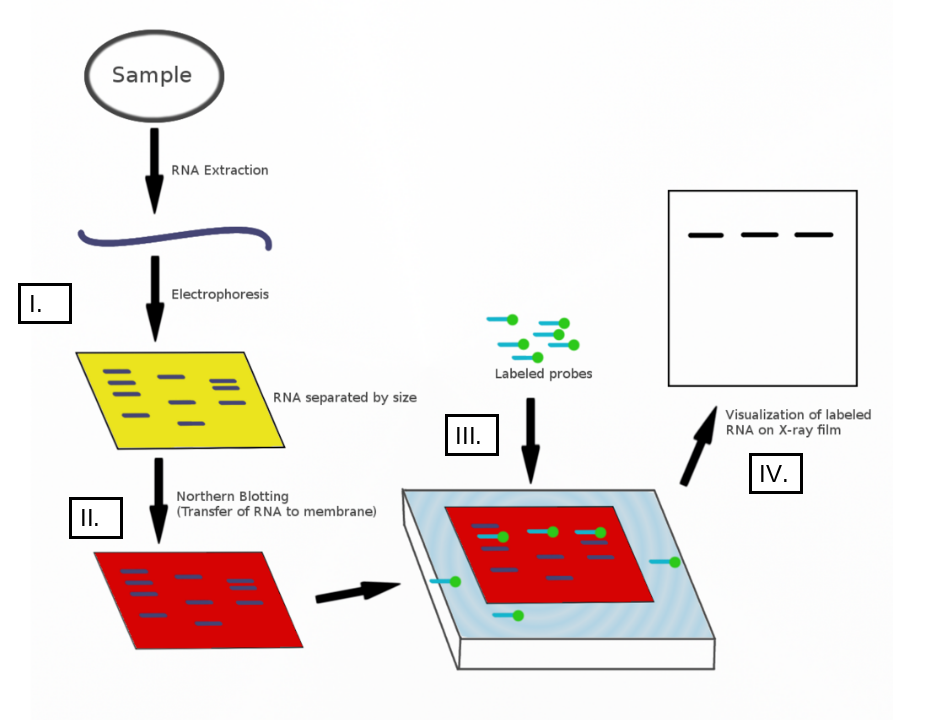
\includegraphics[width=\textwidth]{images/northernblot.png}
    \caption{\textbf{Ablauf eines Northern Blot}: Bei einem Northern Blot wird die durch eine Gelelektrophorese (I.) aufgetrennten RNA auf eine Membran übertragen (II.). Anschließend wird die RNA auf der Membran mit spezifischen und gelabelten Proben hybridisiert (III.) und kann so auf der Filtermembran nachgewiesen werden (IV). }
    \label{fig:northernblot}
\end{figure}
\index{Northern Blot}
\begin{mybox}[title=Unterschied Northern Blot und Southern Blot]%K
Southern Blot ist für DNA und Northern Blot ist für RNA. (Dementsprechend ist natürlich die Isolierung auch anders). \\
Außerdem findet im Nothern-Blot keine Denaturierung und kein Restriktionsenzym-Verdau statt, da RNA bereits einzelsträngig und meistens relativ kurz ist. \index{Northern Blot} \index{Southern Blot}
\end{mybox} 
PSAT = Phosphoserin-Aminotransferase \\
PHGDH = Phosphoglycerat-Dehydrogenase
\begin{mechanism}[title=Wie funktioniert Northern Blot? Und wofür wird es verwendet?]
\begin{enumerate}
    \item DNA-Extraktion und -Aufbereitung (Reinigung)
    \item Gelelektrophorese
    \item Transfer auf eine Membran
    \item Hybridisierung mit einer markierten Sonde
    \item Waschen
    \item Detektieren
\end{enumerate}
Verwendung:  RNA-Moleküle innerhalb einer Probe zu detektieren und zu quantifizieren
\end{mechanism}
\subsection{Reverse Transkriptase PCR (RT-PCR)}
\index{Reverse Transkriptase PCR}
\begin{figure}[H]%K
\centering
    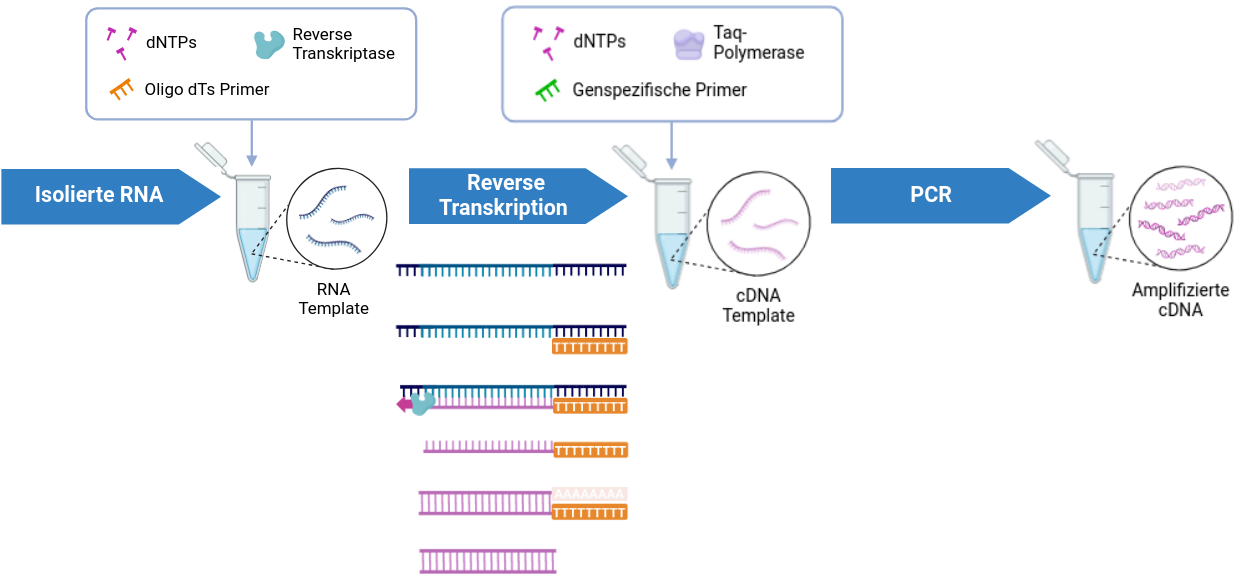
\includegraphics[width=\textwidth]{images/rtpcr.png}
    \caption{\textbf{RT-PCR}: Die extrahierte RNA wird unter der Verwendung von \glspl{dntp} durch \gls{Reverse Transkriptase} in komplementären c(opy)DNA umgeschrieben.  \\ Die RNA wird anschließend via \gls{RNA-Hydrolyse} durch \gls{RNase} H abgebaut. \gls{taq} synthetisiert den komplementären cDNA Strang und die PCR-Reaktion wird gestartet.} \index{RNA-Hydrolyse}
    \label{fig:rtpcr}
\end{figure}
Schritte als Liste: 
\begin{enumerate}
    \item Extraktion von RNA
    \item Synthese einer komplementären c(opy) DNA durch Reverse Transkriptase
    \item RNA-Hydrolyse durch RNase H
    \item Synthese des komplementären cDNA Strangs durch Taq-Polymerase
    \item Start der PCR-Reaktion
\end{enumerate}
\begin{mybox}[title=Was genau ist Real-time quantitative RT-PCR?] %K
Eine Kombination aus RT-PCR und qPCR. Also eine PCR unter Verwendeung einer reversen Transkriptase mit einer Konzentrationsbestimmung in Echtzeit. 
\index{Real-time quantitative RT-PCR} 
\end{mybox}
\noindent Nachweis des PCR-Prouktes via \gls{sybr}: Wenn die Hybridisierung (der Nachweis) klappt, bindet \gls{sybr} an die doppelsträngige DNA. -> Erlaubt Echtzeitmessung und quantitative Analyse! \\ \newline
Auswertung der PCR über die Amplifikationskurve: Fluoreszenzintensität wird nach jedem Zyklus aufgezeichnet und gegen die Zyklusnummer aufgetragen (aka eine Achse des Graphen ist die Fluoreszenzintensität und die andere die Zyklusnummer). \\
Der Ct-Wert (Threshold Cycle) ist der Zyklus, in dem die Fluoreszenzintensität einen definierten Schwellenwert (Threshold) überschreitet. Ist ein Maß für die Menge der ursprünglichen DNA-Vorlage in der Probe. \\ \index{Ct-Wert} \index{Threshold Cycle}
\noindent Floreszenz ensteht übrigens durch den Förster Resonanz Energy Transfer (FRET). \index{Förster Resonanz Energy Transfer}
\begin{mechanism}[title=Wie funktioniert qPCR\, was ist der Ct-Wert und welche mRNA liegt am meisten vor?]
Methode zur quantitativen Messung von DNA (oder RNA als qRT-PCR). \\ Der Ct-Wert ist der Zyklus, bei dem die fluoreszierende Signale die definierte Schwelle (Threshold) überschreiten und somit deutlich über dem Hintergrundrauschen liegen. \\
Ablauf: 
\begin{itemize}
    \item DNA-Extraktion bzw. extrahierte RNA in cDNA transkribieren 
    \item Amplifikation der (c)DNA
    \item Echtzeit-Detektion der Floreszenz während der PCR-Zyklen 
\end{itemize}
In einer qPCR-Analyse wird die mRNA mit dem niedrigsten Ct-Wert als die am meisten vorkommende betrachtet. 
\end{mechanism} \index{qPCR}
 
\begin{table}[H] %K
    \centering
    \begin{tabular}{p{2cm}p{4cm}p{4cm}p{4cm}}
       &  \textbf{qPCR} & \textbf{RT-PCR} & \textbf{qRT-PCR} \\ \\
    \textbf{Ausgangs-material} & DNA & RNA & RNA \\ \\
    \textbf{Methode} & Denaturierung und Amplifikation & Reverse Transkription und Amplifikation & Reverse Transkription und Echtzeit-Amplifikation \\  \\
    \textbf{Polymerase} &  	DNA-Polymerase &  	DNA-Polymerase und Reverse Transkriptase & DNA-Polymerase und Reverse Transkriptase \\ \\
    \textbf{Zweck} & Quantifizierung (DNA) & Nachweis von RNA-Expression (qualitativ) & Quantifizierung von RNA-Expression \\ \\
    \textbf{End-material}& DNA & cDNA & cDNA  \\ \\
    \textbf{Messung} & Echtzeit-Detektion (Fluoreszenz) & Gel-Elektrophorese & Echtzeit-Detektion (Fluoreszenz)
    \end{tabular}
    \caption{Vergleich von verschiedenen PCR-Typen.}
    \label{tab:pcrtypen}
\end{table}
% \subsubsection{PCR und Hybridisierung} TODO?
\subsection{Serial analysis of gene expression} \index{Serial analysis of gene expression}
-> Ziel: Momentaufnahme der mRNA in Form von \glspl{Tag} \\
Ablauf: 
\begin{figure}[H]
\centering
    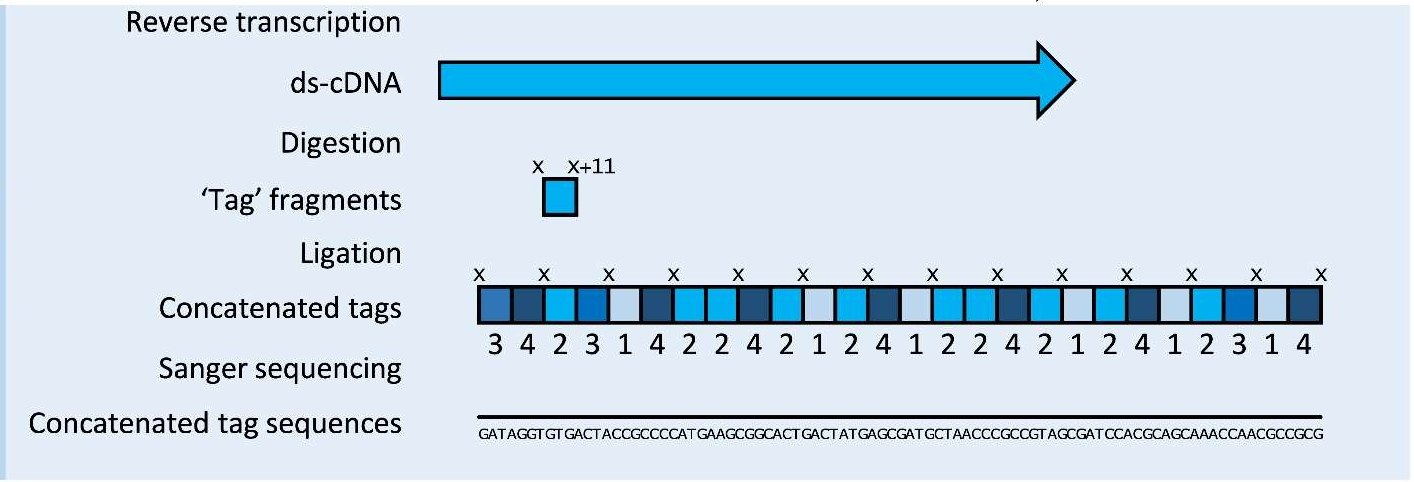
\includegraphics[width=\textwidth]{images/sagepart.jpg}
    \caption{\textbf{SAGE}:}
    \label{fig:sagepart}
\end{figure}
\begin{itemize}
    \item mRNA wird via reverse Transkription in cDNA umgeschrieben 
    \item cDNA wird an Mikrokügelchen gebunden \index{Mikrokügelchen}
    \item Verdau der cDNA durch Restriktionsendonukleasen -> \glspl{Tag}
    \item Tags werden aneinander gereiht (Ligation)
    \item Sanger Sequenzierung der zusammengesetzen \gls{Tag}-Sequenz 
    \item Frequenz der \glspl{Tag} ermitteln  \index{Tag}
\end{itemize}
\begin{mybox}
\begin{itemize} %K
    \item \textbf{in vivo}: im lebenden Organismus
    \item \textbf{in vitro}: außerhalb eines lebenden Organismus, "im Glas"
    \item \textbf{in silico}: computerbasierte Analysen oder Simulationen
\end{itemize}
\end{mybox}
\begin{mybox}[title=Wie läuft eine Verdauung ab?]%K
DNA- oder RNA-Moleküle werden mit Hilfe von Restriktionsenzymen in kleinere Fragmente geschnitten. 
\end{mybox}
\subsection{DNA-Chip Technologie} \index{DNA-Chip} %K
Basiert auf Hybridisierung und Fluoreszenzmarkierungen. \\
Bestandteile: 
\begin{itemize}
    \item mobile Phase: Lösung mit Zielsequenz (fluoreszente Probe) %K
    \item immobile Phase: Trägermaterial mit Sonden (Array) %K
\end{itemize}
\begin{figure}[H] 
    \centering
    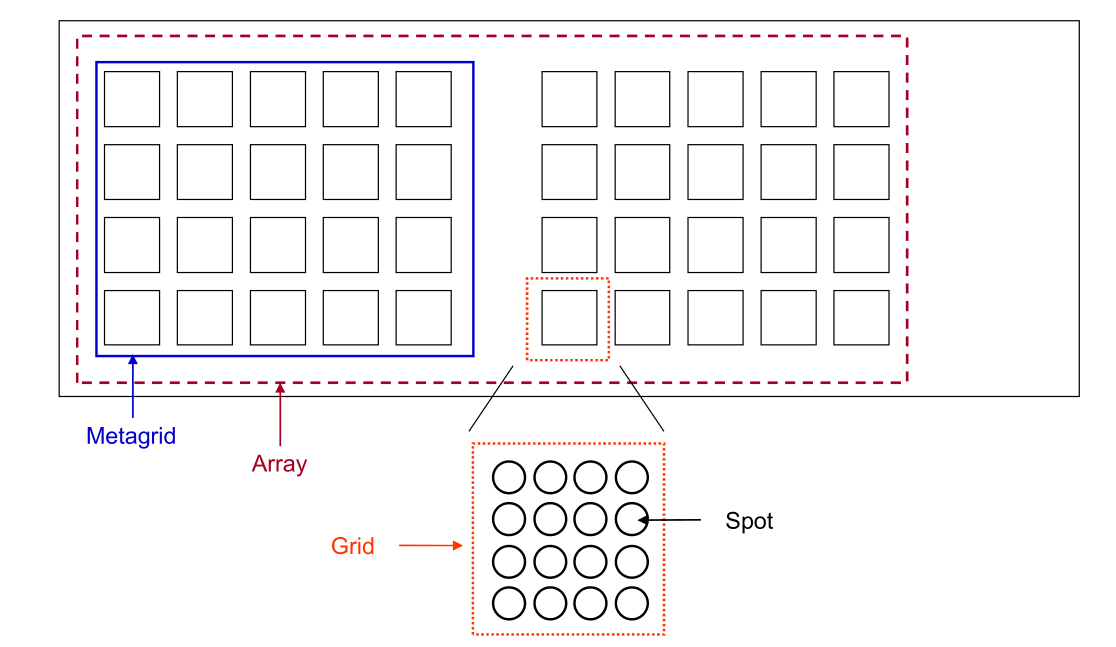
\includegraphics[width=12cm]{images/arrayterms.png}
    \caption{Terminologie des Layout von Arrays.}
    \label{fig:arrayterms}
\end{figure}
Typen: 
\begin{itemize}
    \item \textbf{Macroarray} (High Density Array): \index{Macroarray} \index{High Density Array}
    \begin{itemize}
        \item \textit{Herstellung}: Auftragen von \glspl{Oligonukleotid}n oder PCR Fragmenten
        \item \textit{Substrate}: Membranen 
    \end{itemize}
    \item \textbf{Microarray}:  \index{Microarray}
    \begin{itemize}
        \item \textit{Herstellung}: Auftragen von \glspl{Oligonukleotid}n oder PCR Fragmenten
        \item \textit{Substrate}: Glas etc. 
    \end{itemize}
    \item \textbf{Chip}:  
    \begin{itemize}
        \item \textit{Herstellung}: Synthese auf dem Träger
        \item \textit{Substrate}: Glas etc. 
    \end{itemize}
\end{itemize}
\subsubsection{Microarray} \index{Microarray}
\subsubsection{Herstellung}
Auftragen von \glspl{Oligonukleotid}n oder PCR Fragmenten / Synthese geht durch:
\begin{itemize}
            \item \textbf{Photolithographische Festphasensynthese}: 
            \begin{itemize} \index{Photolithographische Festphasensynthese}
                \item \textit{Steuerung der Synthese}: \glspl{photolithografisch Methode}
                \item \textit{Bindungsprozess}: \glspl{photolithografisch Methode}
                \item \textit{Flexibilität}: Hoch, Reihenfolge der Synthese der Sonden kann gesteuert werden
            \end{itemize}
            \item \textbf{Agilent-Verfahren}: 
            \begin{itemize} \index{Agilent-Verfahren}
                \item \textit{Steuerung der Synthese}: \glspl{photolithografisch Methode}
                \item \textit{Bindungsprozess}: \glspl{photolithografisch Methode}
                \item \textit{Flexibilität}: Hoch, einzelne Sonden können angepasst werden 
            \end{itemize}
            \item \textbf{Immobilisierung vorgefertigter DNA auf dem Chip}: 
            \begin{itemize}
                \item \textit{Steuerung der Synthese}: DNA wird vor dem Aufbringen synthetisiert 
                \item \textit{Bindungsprozess}: chemische Wechselwirkungen zwischen der DNA und der Chip-Oberfläche
                \begin{itemize}
                    \item Größere DNA-Moleküle: elektrostatische Wechselwirkungen
                    \item Kleinere DNA-Moleküle: kovalente Bindung
                \end{itemize}
                \item \textit{Flexibilität}: Eingeschränkt auf vorgefertigte DNA 
            \end{itemize}
        \end{itemize}


\subsubsection{Differentielle Expressionsanalyse}%K \index{Expressionsanalyse!Differentielle}
Unterschiede in der Genexpression zwischen verschiedenen Bedingungen, Behandlungen oder Gruppen identifizieren und quantifizieren. \\
Methoden: 
\begin{itemize}
    \item RNA-Sequenzierung \index{RNA-Sequenzierung}
    \item \textbf{Microarrays} \index{Microarrays}
    \begin{enumerate}
        \item RNA isolieren
        \item in cDNA umschreiben 
        \item cDNA mit Floreszenzstoffen markieren 
        \item Hybridisierung auf den Chip 
    \end{enumerate}
    \item Quantitative PCR (qPCR)
\end{itemize}

\subsubsection{Readout}
\begin{figure}[H]
    \centering
    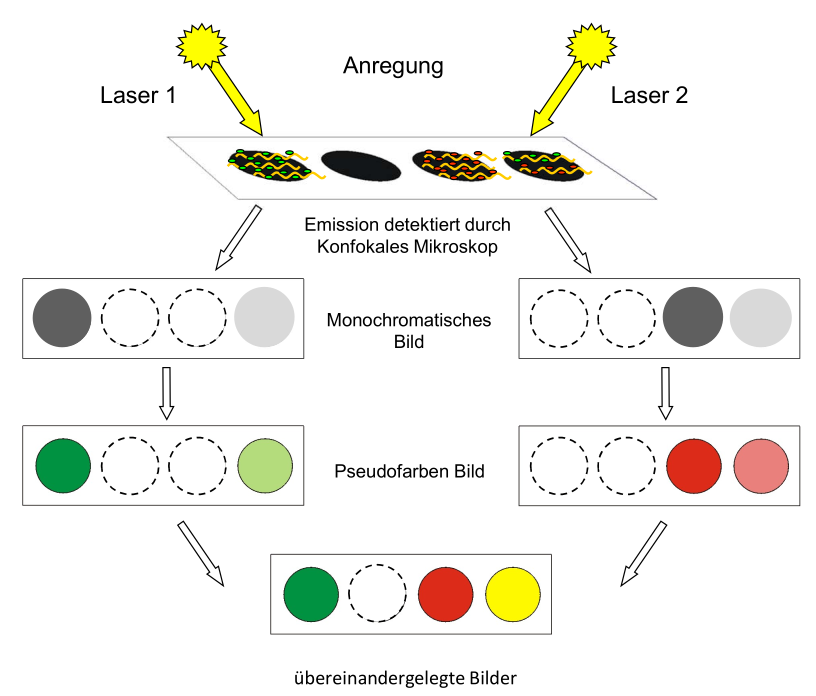
\includegraphics[width=12cm]{images/readout.png}
    \caption{Die eingebauten Fluoreszenzstoffe werden durch Laserlicht angeregt und die Emission mit Hilfe eines Konfokalen Laser Scanningmikroskops gemessen.}
    \label{fig:readout}
\end{figure}



\subsection{Transkriptomsequenzierung / RNAseq} \index{RNAseq}
\begin{mechanism}[title=Was versteht man unter dem Begriff RNAseq?]
RNA-Sequenzierung - quantitative Methode zur Analyse des Transkriptoms eines Organismus.
\end{mechanism}
\begin{mechanism}[title=Erläutern Sie das Prinzip der RNAseq und skizzieren Sie den Workflow]
Prinzip: RNA-Moleküle in cDNA umzuschreiben und diese dann zu sequenzieren  \\
Workflow: 
\begin{enumerate}
    \item RNA Isolierung
    \item (RNA Fragmentierung)
    \item cDNA Synthese
    \item Sequenzierung
    \item (weitere Analyse)
\end{enumerate}
\end{mechanism}
quantitativ \\
Ziel: Identifizierung \textbf{aller} Arten von Transkripten \\

\subsubsection{RNAseq bei Bakterien} \index{RNAseq!bakterielle}
-> schwierig, denn in Bakterien gibt es keine Poly-A-Schwänze an der mRNA (werden gezielt abgebaut) \\
-> Bakterien haben viel rRNA, die muss entfernt werden, dmait man die \textbf{mRNA} untersuchen kann \\
-> Alternative ist Bindung der rRNA an magnetische beads über dort immobilisierte anti-rRNA-Oligonukleotide (RiboZeroTM)
\begin{figure}[H]
    \centering
     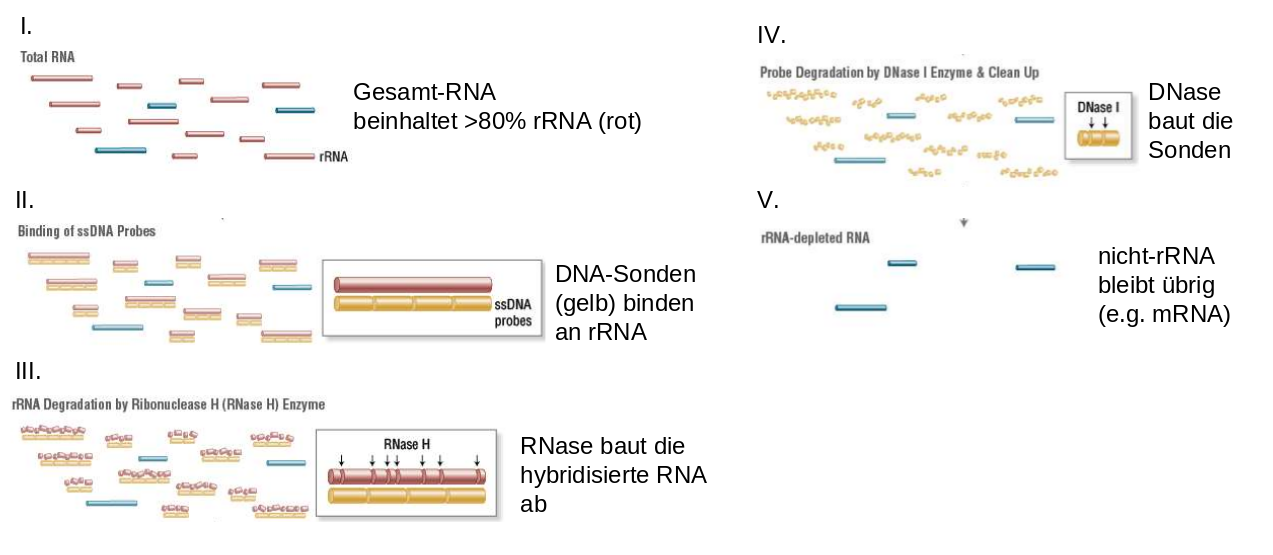
\includegraphics[width=\textwidth]{images/rrnaabbau.png}
    \caption{\textbf{Abbau der rRNA durch Hybridisierung}: Man kann komplementäre Sonden nutzen, um rRNA zu binden und und die doppelsträngigen Hybride abbauen lassen. Dadurch bleiben nur noch die nicht-rRNAs übrig und man kann diese analysieren.}
    \label{fig:rrnaabbau}
\end{figure}
\begin{figure}[H]
\centering
    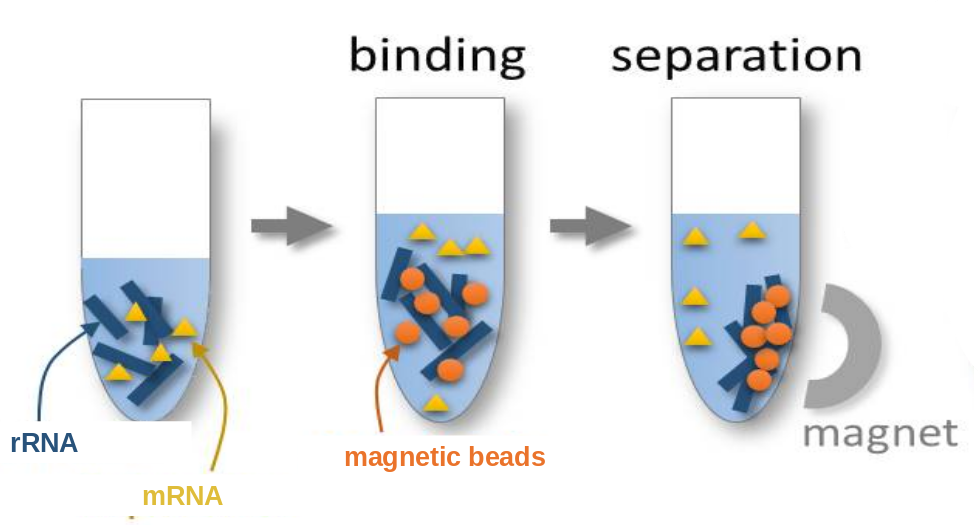
\includegraphics[width=8cm]{images/rRNAextraction.png}
    \caption{\textbf{Abbau der rRNA durch magnetische Beads}: rRNA wird über dort immobilisierte anti-rRNA-\glspl{Oligonukleotid} an magnetische Beads gebunden und somit vom Rest der Lösung getrennt. Die weiterhin freie mRNA kann isoliert werden.}
    \label{fig:rRNAextraction}
\end{figure}

\subsubsection{RNAseq bei Eukaryonten} \index{RNAseq!eukaryotische}
\begin{figure}[H]
    \centering
\begin{subfigure}[t]{0.45\textwidth}
    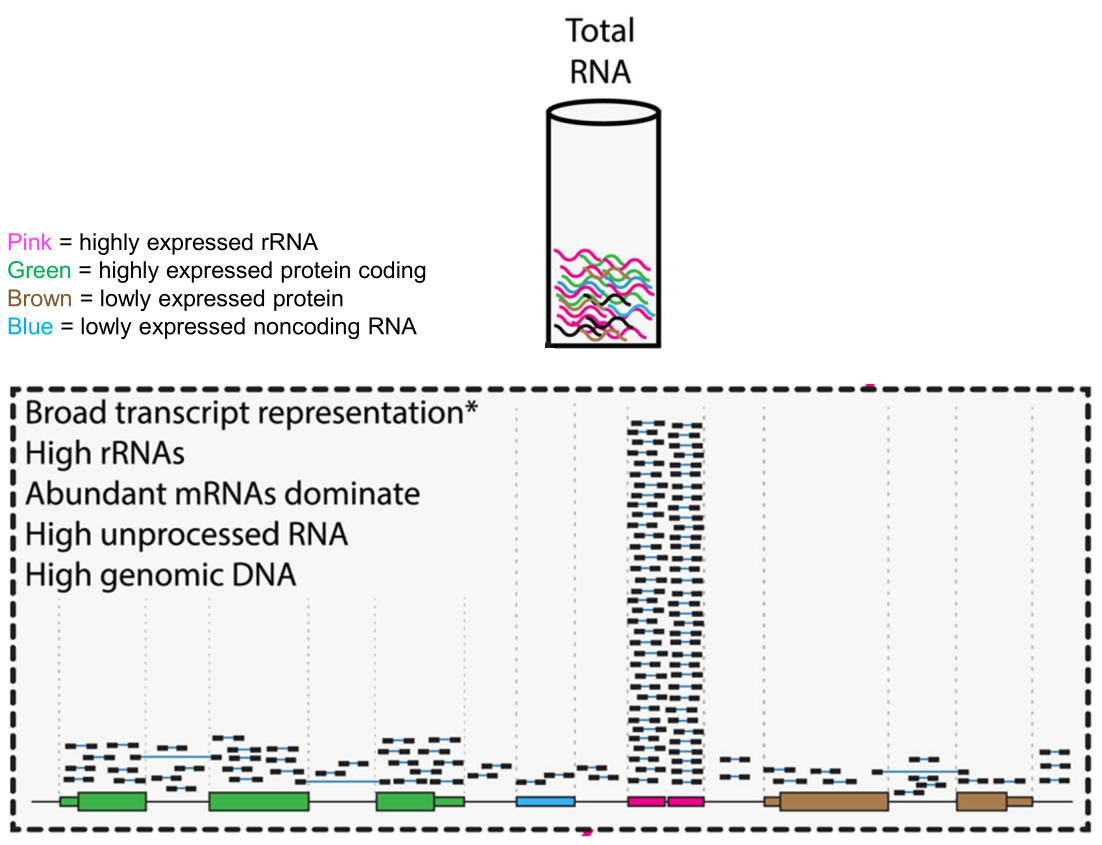
\includegraphics[width=\textwidth]{images/totalrna.png}
    \caption{\textbf{Alle RNA-Typen} identifizieren und Kartieren. Führt dazu, dass die rRNAs das Ergebnis deutlich dominieren.}
    \label{fig:totalrna}
\end{subfigure}
\hfill
\begin{subfigure}[t]{0.45\textwidth}
    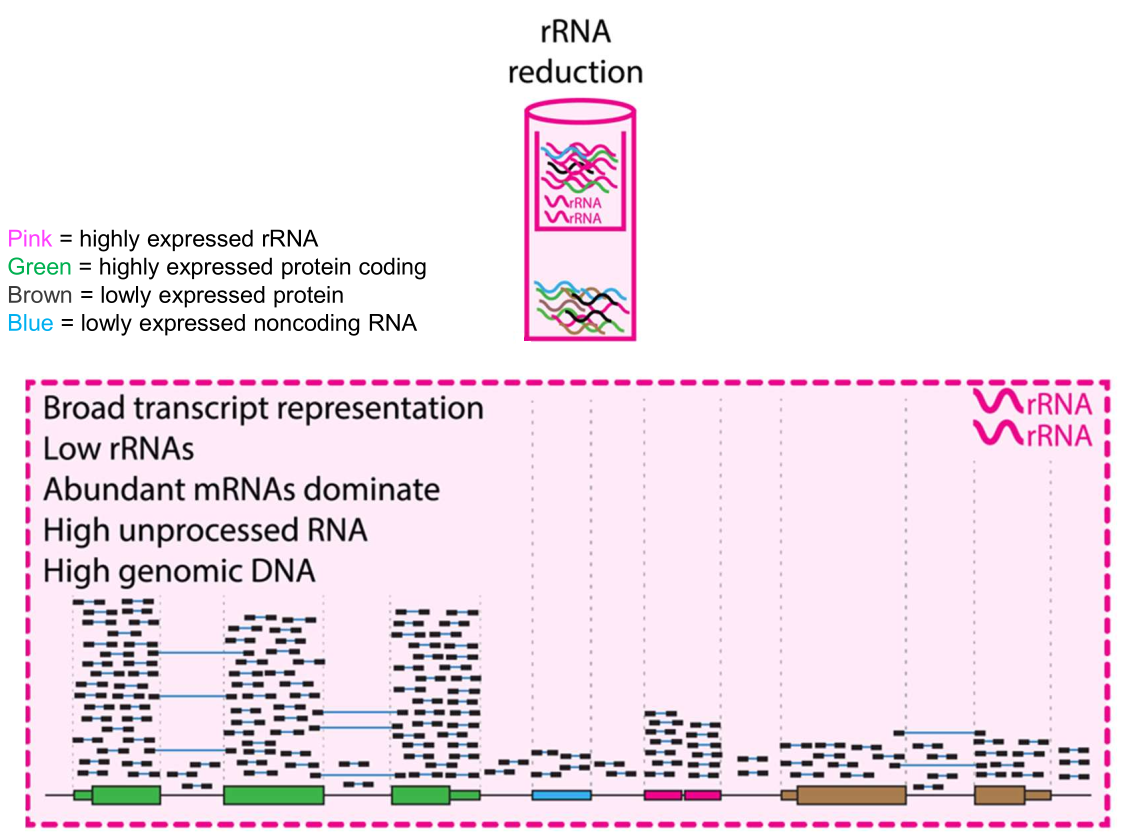
\includegraphics[width=\textwidth]{images/rrna.png}
    \caption{\textbf{Alle RNA-Typen} identifizieren und Kartieren, jedoch mit vor der Analyse deutlich reduzierter ANzahl der rRNA, damit der Fokus auf der mRNA liegt.}
    \label{fig:rrna}
\end{subfigure}
\hfill
\begin{subfigure}[t]{0.45\textwidth}
    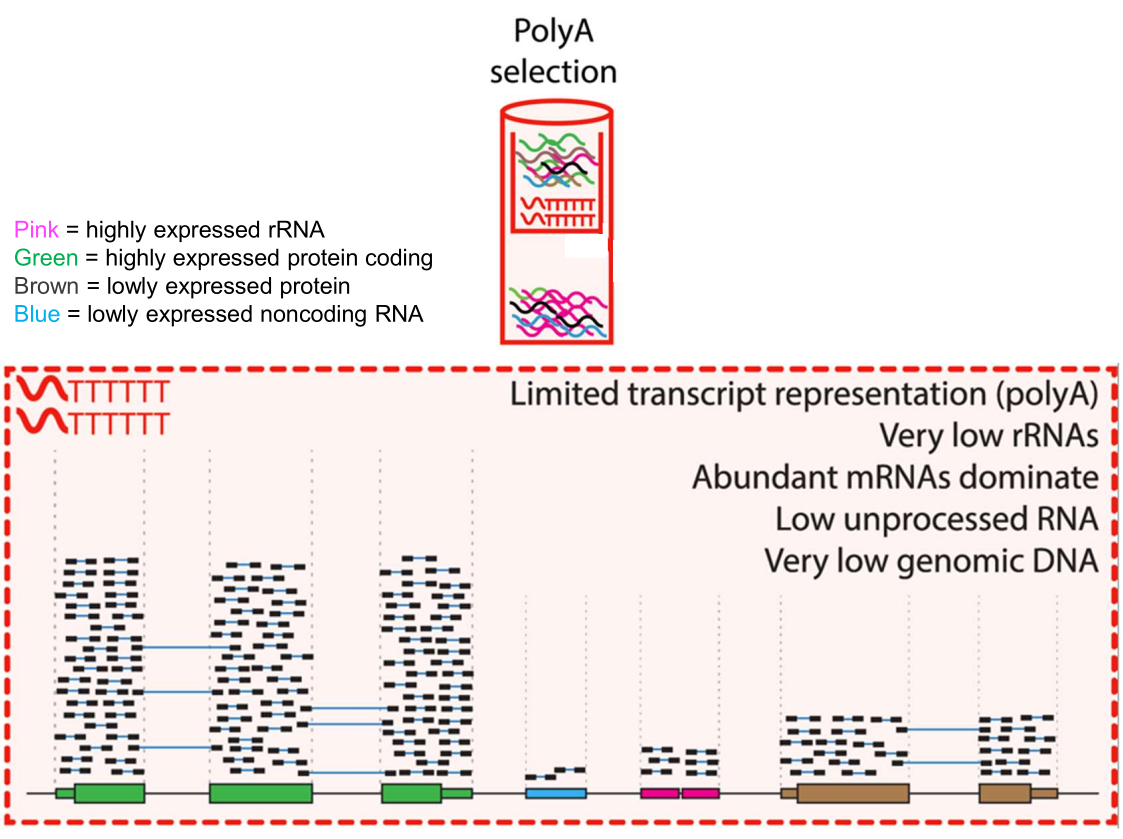
\includegraphics[width=\textwidth]{images/polyarna.png}
    \caption{ \textbf{Genexpressionsanalyse} durch gezielte Analyse der mRNA, indem diese gezielt über ihren Poly-A-Schwanz isoliert wird.}
    \label{fig:polyarna}
\end{subfigure}
    \caption{RNAseq Strategien in Eukaryonten.}
    \label{fig:eukarrnaseq}\index{RNAseq!eukaryotische}
\end{figure}

\subsubsection{Auswertung von RNAseq} \index{RNAseq!Auswertung von}
Reads werden auf ein Referenzgenom kartiert (den entsprechenden Positionen zugeordnet) und erzeugen so eine „Landschaft“ (transcriptional landscape, transcriptional profile) aus der man ableiten kann, welche Gene aktiv exprimiert werden und in welchen Mengen sie exprimiert werden. \\ \index{transcriptional landscape} \index{transcriptional profile}
Das kann man, wenn Quantitative Strategien die Anzahl von reads berechnen, normalisiert auf die Genlänge und die Gesamtzahl der reads im Experiment (\gls{rpkm}). \index{Reads Per Kilobase of gene per Millions of total reads}
\begin{mybox}[title=Warum Normalisierung?]
 Die Rohzählungen der Reads können von verschiedenen Faktoren beeinflusst werden, wie z.B. der Gesamtmenge an RNA in der Probe, der Effizienz der Sequenzierung und der Länge der Gene. Um die Daten vergleichbar zu machen, sind Normalisierungsverfahren erforderlich.
\end{mybox}
\section{Scatter plot} \index{Scatter plot}
Scatter plots werden verwendet, um die Beziehung zwischen zwei verschiedenen kontinuierlichen Variablen zu bewerten. In diesen Diagrammen werden Veränderungen bei zwei verschiedenen Variablen gleichzeitig verglichen (daher keine durchgehende Linie).  
\begin{figure}[H]
    \centering
    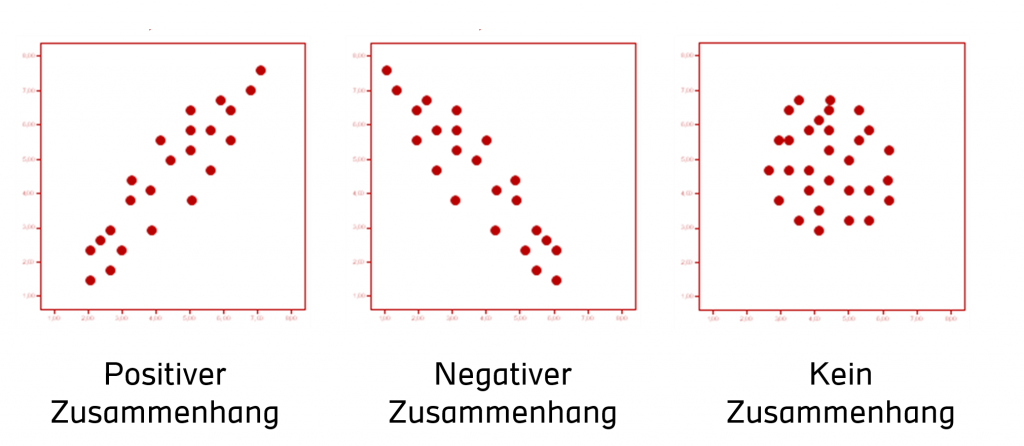
\includegraphics[width=12cm]{images/plotarten.png}
    \caption{Man kann visuell erkennen, ob ein positiver, negativer oder kein Zusammenhang zwischen den beiden Variablen besteht.}
    \label{fig:plotarten}
\end{figure}
\subsection{M/A-Plots} \index{M/A-Plots}
-> Unterschiede in der Genexpression zwischen zwei Bedingungen oder Proben visuell darstellen
\begin{itemize} 
    \item \textbf{M-Achse}: zeigt an, wie viel mehr oder weniger ein Gen in einer Bedingung im Vergleich zur anderen Bedingung exprimiert wird
    \begin{itemize}
        \item Positiv: Gen wird in der zweiten Bedingung stärker exprimiert
        \item Negativ: Gen wird in der ersten Bedingung stärker exprimiert
    \end{itemize}
    \item \textbf{A-Achse}: zeigt die durchschnittliche Expression des Gens in beiden Proben
\end{itemize}

%FISH gab es ja schon
\begin{mechanism}[title=Sie wollen die Genexpression in einer prokaryotischen Zelle quantitativ und qualitativ messen.\\ Wie gehen Sie vor?]
Als Qualitative Analyse führt man eine RT-PCR durch, um herauszufinden, ob ein Gen in der Probe exprimiert wird. \\
Als quantitative Analyse führt man eine qPCR mit anschließender RNAseq durch.  \\ \newline
Man kann auch direkt eine RT-qPCR durchführen und anschließend eine RNAseq. 
\end{mechanism}

\section{Räumliche Transkriptomik}%K
Räumliche Transkriptomik (spatial transcriptomis) oder räumlich aufgelöste Transkriptomik ist eine Methode, die den Positionskontext der Transkriptionsaktivität in intaktem Gewebe erfasst. \\
Es umfasst einen wichtigen Teil der räumlichen Verteilung von biologischen Molekülen in Geweben.
